%*
%* Seven Kingdoms: Ancient Adversaries
%*
%* Copyright 1997,1998 Enlight Software Ltd.
%* Copyright 2018 Timothy Rink
%*
%* This program is free software: you can redistribute it and/or modify
%* it under the terms of the GNU General Public License as published by
%* the Free Software Foundation, either version 2 of the License, or
%* (at your option) any later version.
%*
%* This program is distributed in the hope that it will be useful,
%* but WITHOUT ANY WARRANTY; without even the implied warranty of
%* MERCHANTABILITY or FITNESS FOR A PARTICULAR PURPOSE.  See the
%* GNU General Public License for more details.
%*
%* You should have received a copy of the GNU General Public License
%* along with this program.  If not, see <http://www.gnu.org/licenses/>.
%*
%*

\chapter{Developing Weapons}

\index{weapons!developing}

\section{Towers of Science}

\index{towers of science}

\begin{wrapfigure}{l}{0.3\textwidth}
	\vspace{-20pt}
	\begin{center}
		
\includegraphics[width=0.3\textwidth]{Itower} % Original size.
		\\ Tower of Science
	\end{center}
	\vspace{-20pt}
\end{wrapfigure}

% Hyphenation here

\textgoth{\Huge{W}}ithout the benefits of Towers of Science, you may as well resign yourself to a landlocked Empire known for sending its ill-equipped Soldiers into the mouths of enemy cannon. Put to use the benefits of research, however, and your Empire will become feared far and wide.

Researchers may be assigned to the Towers of Science in the same way that workers are assigned to factories. Peasants trained in Research or skilled researchers hired in Inns are the most useful. Over time, your scientists will acquire great skill and speed in their studies. They will become a most precious asset and must be protected accordingly.

% Tower of Science is shortened to Tower

You are not limited to one Tower of Science. It is most advisable to have more than one working on either the same or different projects simultaneously. All Towers of Science will share information so that if you begin a research project in a new Tower, your researchers will start at the level that the other Towers have reached.

\clearpage

\subsection{Choosing Technology to Research}

\index{researching weapons}
\index{weapons!research}

\begin{wrapfigure}{r}{0.4\textwidth}
	\vspace{-20pt}
	\begin{center}
		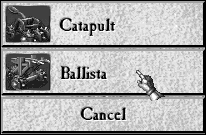
\includegraphics[width=0.4\textwidth]{Iresearch_begin} % Original size.
	\end{center}
	\vspace{-20pt}
\end{wrapfigure}

\textgoth{\Huge{W}}hen selected, a Tower of Science will show a list of weapons and naval technologies that at this time have a possibility of being researched. Choose a Weapon or Ship, and your scientists will immediately get to work on developing it.

The bar moving from left to right shows the progress of that research.

When the research is complete, you will hear the announcement, \\ % FIXES AN OVERFLOW
“\textbf{\textit{Research project is complete}}.” You should then go to your Tower of Science to start immediately on a new project.

All weapons and ships, when fully researched, will immediately become available for production in your War Factories or Harbors.

\subsection{Weapon Levels}

\index{weapons!levels}

\textgoth{\Huge{M}}ost Weapon technologies can be researched to three levels: \textbf{Mark I}, \textbf{Mark II}, and \textbf{Mark III}. As soon as the research is complete at the Mark I level, your researchers will immediately begin on Mark II unless you order them otherwise.

\begin{center}
	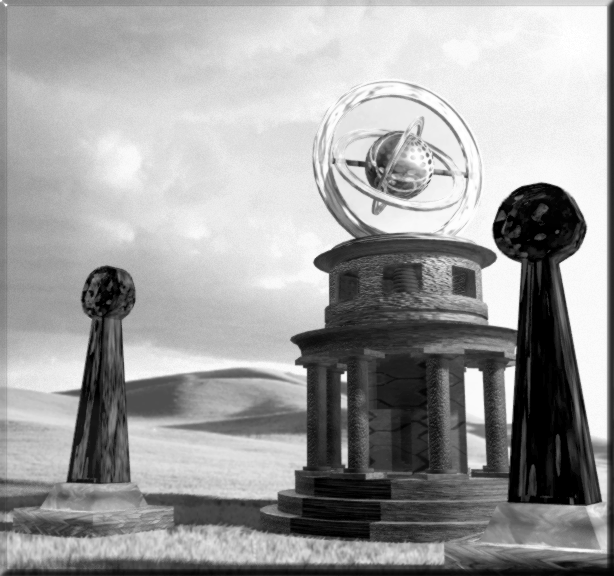
\includegraphics[width=0.85\linewidth]{Atower} % Original size?
\end{center}

% F6 is bold.

To view the progress of research at all Towers of Science, press the \textbf{F6} key.

\section{War Factories}

\index{war factories}

\begin{wrapfigure}{l}{0.3\textwidth}
	\vspace{-20pt}
	\begin{center}
		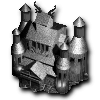
\includegraphics[width=0.3\textwidth]{Iwarfactory} % Original size.
		\\ War Factory
	\end{center}
	\vspace{-30pt}
\end{wrapfigure}

\textgoth{\Huge{W}}ar Factories produce those Weapons that are so necessary in keeping the peace. To assign workers to the War Factory, follow the same procedure as in an ordinary Factory. The skill of the workers will be reflected in the speed of Weapons production. \\ \\ %

\subsection{Make Weapon}

\index{creating!weapons in war factory}
\index{weapons!creating in war factory}

\begin{wrapfigure}{r}{0.1\textwidth}
	\vspace{-20pt}
	\begin{center}
		
\includegraphics[width=0.1\textwidth]{Tweaponmake}
	\end{center}
	\vspace{-20pt}
\end{wrapfigure}

\textgoth{\Huge{W}}hen the War Factory is selected, \textbf{Click} on the \textbf{Make Weapon Tile}.

% (See Tower of Science): I want this to be bold type.

You must then choose the type of Weapon that you want to build. Your choices will depend on the Weapons that you have researched. (See Tower of Science). If you have not yet researched any Weapons, you will be unable to build anything.

\subsubsection{Producing a Single Weapon}

\textbf{\textgoth{\Huge{C}}lick} on the name of the weapon that you want to produce. You will then exit the menu, and production will begin. The Weapon will exit the War Factory when production is finished.

\subsubsection{Production Queue}

\textgoth{\Huge{T}}o the right of the Weapon’s name, you will see the number 0. \textbf{Click} on this repeatedly until you see the number of Weapons that you want to build. If you wish to decrease the number, you may \textbf{Right-Click} on it.

Once you have researched more than one type of Weapon, you may select any number and combination of Weapons and produce them in the order that they were selected.

When you have entered the quantity for all of your desired Weapons, \textbf{Click} on the \textbf{Done Button}. When you do, production will begin on one Weapon at a time in the order that you \textbf{Clicked} on their numbers.

As each Weapon is finished, it will exit the War Factory.

\subsubsection{Weapons Hit-Points}

\index{weapons!hit points}

% Hyphenation here.

\textgoth{\Huge{W}}eapons, like Soldiers, have a certain number of Hit-Points. These differ for each kind of Weapon. When a weapon has lost some Hit-Points in fighting, those Hit-Points can be restored by leaving the Weapon at rest. They will be restored twice as fast if the Weapons are assigned to a Fort.

\begin{center}
	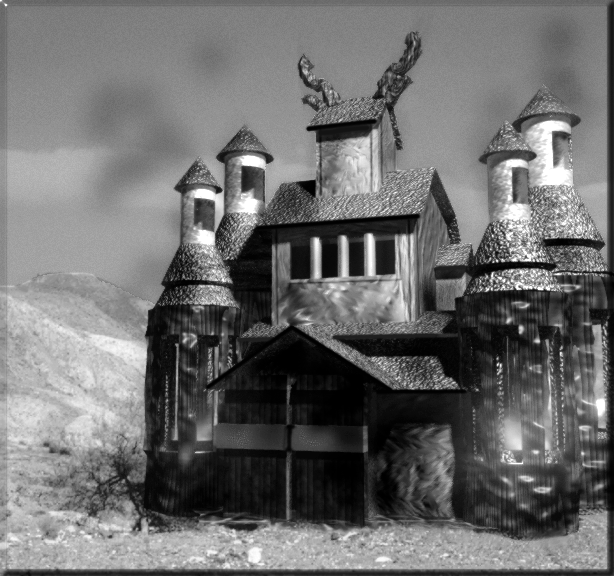
\includegraphics[width=0.7\linewidth]{Awarfactory} % Original size?
\end{center}

\clearpage

\section{Weapons}

\index{weapons!characteristics}

\begin{center}
	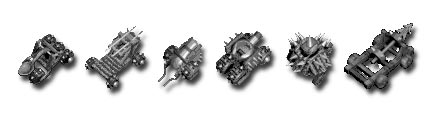
\includegraphics[width=1\linewidth]{Iweapons} % Original size?
	\\ Catapult Ballista Cannon Spitfire Porcupine Unicorn
\end{center}

\subsection{Catapults}

\index{catapults}

\begin{tabular}{p{1.264in} p{1.264in} p{1.264in}}
Yearly Cost: 50. & Hit-Points: 50. & Targets: Ground and Sea.
\end{tabular}

\begin{tabular}{|p{1.264in} p{1.264in} p{1.264in}|}
	\hline
	\textbf{Mark I}	& \textbf{Mark II} & \textbf{Mark III} \\
	Stone Projectile & Naphtha Projectile & Naphtha Projectile \\
	Range 1-7 & Range 1-7& Range 1-7 \\
	Damage Low & Damage Medium & Damage High \\
	\hline
\end{tabular}

\begin{wrapfigure}{r}{0.6\textwidth}
	\vspace{-20pt}
	\begin{center}
		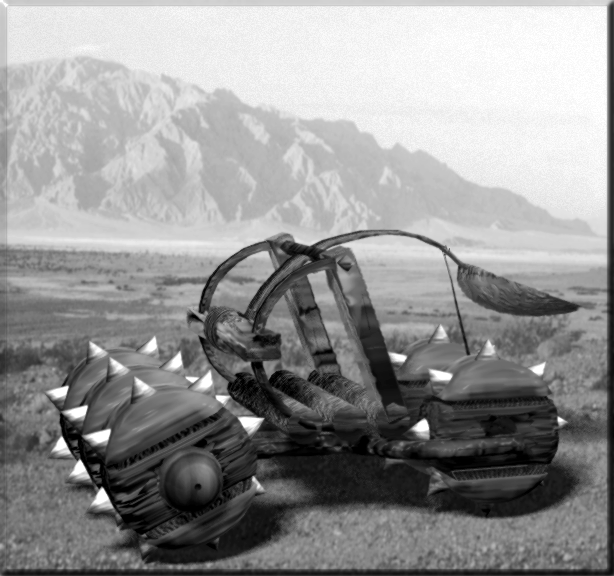
\includegraphics[width=0.6\textwidth]{Acatapult} % Original size.
	\end{center}
	\vspace{-20pt}
\end{wrapfigure}

\textgoth{\Huge{C}}atapults are your most basic weapon of defense. 

There are no prerequisites for researching Catapults. 

You will need to research Catapults before you can research the Spitfires.

\clearpage

\subsection{Ballistae}

\index{ballistae}

\begin{tabular}{p{1.264in} p{1.264in} p{1.264in}}
	Yearly Cost: 60. & Hit-Points: 60. & Targets: Ground, Sea, and Air.
\end{tabular}

\begin{tabular}{|p{1.264in} p{1.264in} p{1.264in}|}
	\hline
	\textbf{Mark I}	& \textbf{Mark II} & \textbf{Mark III} \\ 
	Range 1-7 & Range 1-7& Range 1-7 \\ 
	Speed Slow & Speed Medium & Speed High \\ 
	\hline
\end{tabular}

\begin{wrapfigure}{r}{0.6\textwidth}
	\vspace{-20pt}
	\begin{center}
		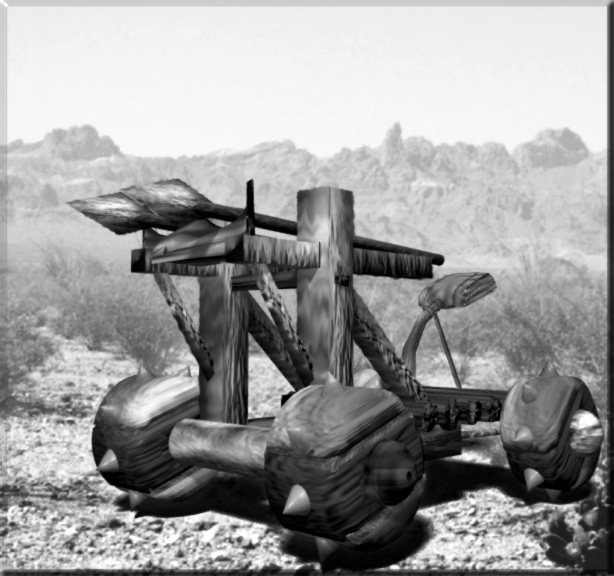
\includegraphics[width=0.6\textwidth]{Aballista} % Original size.
	\end{center}
	\vspace{-20pt}
\end{wrapfigure}

\textgoth{\Huge{Y}}our Ballistae are a step up from the Catapults.

You may, however, find a higher Mark Catapult to be more deadly than a lower Mark Ballista.

There are also no prerequisites for the research of Ballistae.

You will need to research Ballistae before you can research Cannon.

\clearpage

\subsection{Cannon}

\index{cannon}

% Add hspace

\begin{tabular}{p{1.264in} p{1.264in} p{1.264in}}
	Yearly Cost: 80. & Hit-Points: 60. & Targets: Ground, Sea, and Air.
\end{tabular}

\begin{tabular}{| p{1.264in} p{1.264in} p{1.264in}|}
	\hline
	\textbf{Mark I}	& \textbf{Mark II} & \textbf{Mark III} \\ 
	Range 1-6 & Range 1-7 & Range 1-8 \\ 
	Damage Low & Damage Medium & Damage High \\ 
	\hline
\end{tabular}
   
\begin{wrapfigure}{r}{0.6\textwidth}
	\vspace{-20pt}
	\begin{center}
		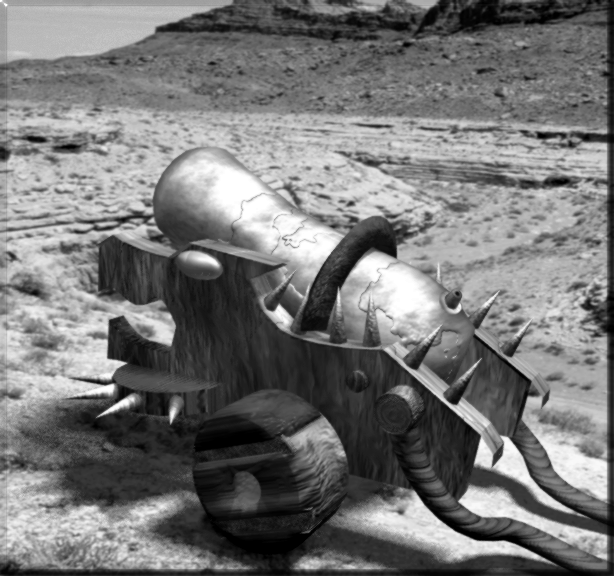
\includegraphics[width=0.6\textwidth]{Acannon} % Original size.
	\end{center}
	\vspace{-50pt}
\end{wrapfigure}

\textgoth{\Huge{A}}fter the Mark II Ballista has been researched, you will be able to begin the researching of the Cannon.

Nothing makes an impression on your foes better than a barrage from the mouths of a dozen Cannon.

\clearpage

\subsection{Spitfires}

\index{spitfires}

\begin{tabular}{p{1.264in} p{1.264in} p{1.264in}}
	Yearly Cost: 70. & Hit-Points: 50. & Targets: Ground and Sea.
\end{tabular}

\begin{tabular}{| p{1.264in} p{1.264in} p{1.264in}|}
	\hline
	\textbf{Mark I}	& \textbf{Mark II} & \textbf{Mark III} \\ 
	Range 1-6 & Range 1-7 & Range 1-8 \\ 
	Damage Low & Damage Medium & Damage High \\ 
	\hline
\end{tabular}

\begin{wrapfigure}{r}{0.6\textwidth}
	\vspace{-20pt}
	\begin{center}
		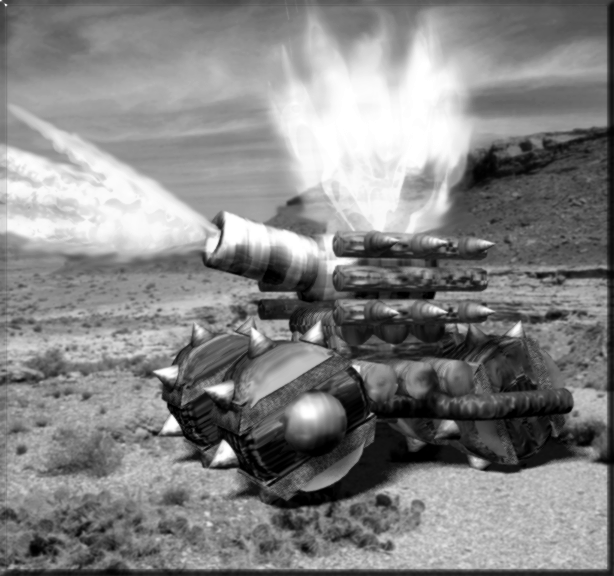
\includegraphics[width=0.6\textwidth]{Aspitfire} % Original size.
	\end{center}
	\vspace{-20pt}
\end{wrapfigure}

\textgoth{\Huge{S}}pitfires ensure that the Soldiers of your foes are given a warm reception whenever they stop by.

You must have researched the Mark II Catapult in order to begin research on the Spitfire. 

You will need to research Spitfires before you can begin research on Porcupines.

\clearpage

\subsection{Porcupines}

\index{porcupines}

\begin{tabular}{p{1.264in} p{1.264in} p{1.264in}}
Yearly Cost: 50. & Hit-Points: 10. & Targets: Ground.
\end{tabular}

\begin{wrapfigure}{r}{0.6\textwidth}
	\vspace{-20pt}
	\begin{center}
		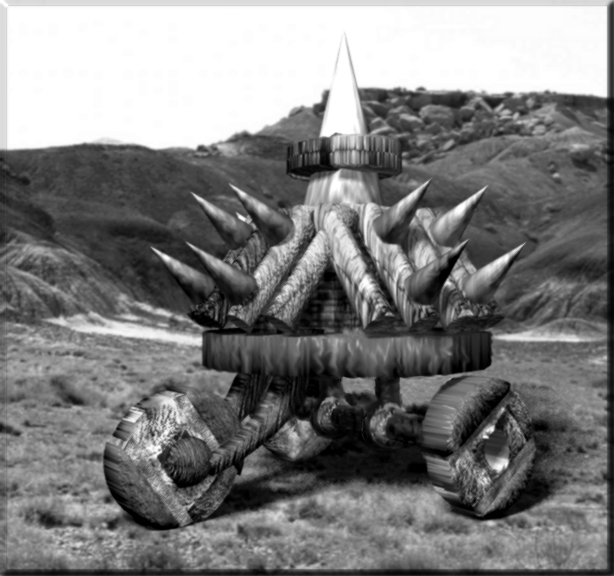
\includegraphics[width=0.6\textwidth]{Aporcupine} % Original size.
	\end{center}
	\vspace{-20pt}
\end{wrapfigure}

\textgoth{\Huge{T}}he Porcupine is a Weapon that, when used correctly and in ample numbers, can wreak havoc on enemy formations and buildings.

It is a Weapon designed to be destroyed by you. Send one or many to a targeted area. When they arrive, fire on them with a Cannon, Catapult, Spitfire, or arrowed soldier. When one of them has been hit by your fire, it will explode, sending its sharp projectiles into your foes.

% Keys here.

To fire on a Porcupine, you must first select at least one Cannon, Catapult, Spitfire, or arrowed soldier. Then hold down the Shift Key on your keyboard. \textbf{Right-Click} on one of your Porcupines to launch the attack.

% Hyphenation here. in ?

When used in large, close-knit formations, the explosion of one will cause a chain reaction explosion in the others of the group. Although Porcupines may be easily destroyed by your enemies, they will not explode, so do not fear keeping them near your other units. You will be unable to research Porcupines until you have completed your research on the Mark II Spitfire.

\clearpage

\subsection{Unicorns}

\index{unicorns}

\begin{tabular}{p{1.264in} p{1.264in} p{1.264in}}
	Yearly Cost: 110. & Hit-Points: 60. & Targets: Ground and Sea.
\end{tabular}

\begin{tabular}{|p{1.264in} p{1.264in} p{1.264in}|}
	\hline
	\textbf{Mark I}	& \textbf{Mark II} & \textbf{Mark III} \\ 
	Range 7	& Range 7 & Range 7 \\ 
	Damage Medium & Damage High & Damage High \\ 
	\hline
\end{tabular}

\begin{wrapfigure}{r}{0.6\textwidth}
	\vspace{-20pt}
	\begin{center}
		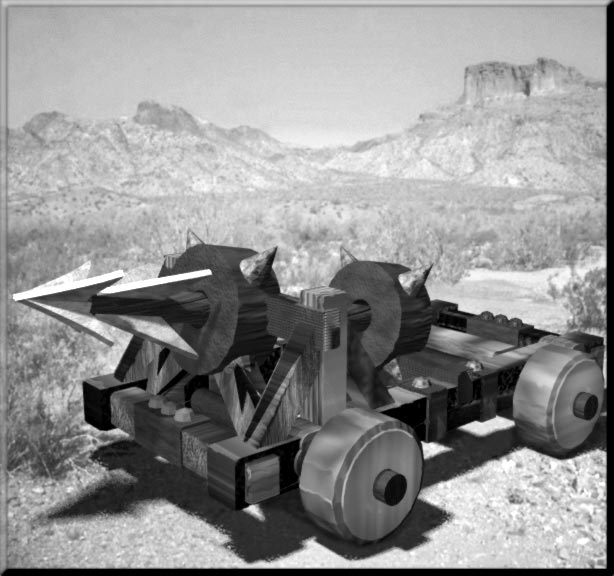
\includegraphics[width=0.6\textwidth]{Aunicorn} % Original size.
	\end{center}
	\vspace{-20pt}
\end{wrapfigure}

\textgoth{\Huge{Y}}ou may research Unicorns only after you have finished your research on the Porcupines.

Unicorns offer your army a powerful weapon with an extremely rapid rate of fire.

% Author's voice.

It is not unknown for an attacking army to lose every single man before coming within striking distance of a line of Unicorns.